\documentclass{article} % For LaTeX2e
%\documentstyle[nips12submit_e,times,art10]{article} % For LaTeX 2.09
\usepackage{nips12submit_e,times,graphicx}
\usepackage{epstopdf}
\nipsfinaltrue
\usepackage[linesnumbered]{algorithm2e} 
\newcommand{\floe}{\emph{Floe }}

\graphicspath{{./figures/}}
\DeclareGraphicsExtensions{.eps}

\title{Distributed Online Clustering using LSH over Multiple Data Streams}

\author{
Alok Kumbhare \\
Department of Computer Science \\
University of Southern California \\
Los Angeles, CA 90007 \\
\texttt{kumbhare@usc.edu} \\
\And
Ketan Singh \\
Department of Computer Science \\
University of Southern California \\
Los Angeles, CA 90007 \\
\texttt{ketansin@usc.edu} \\
}

% The \author macro works with any number of authors. There are two commands
% used to separate the names and addresses of multiple authors: \And and \AND.
%
% Using \And between authors leaves it to \LaTeX{} to determine where to break
% the lines. Using \AND forces a linebreak at that point. So, if \LaTeX{}
% puts 3 of 4 authors names on the first line, and the last on the second
% line, try using \AND instead of \And before the third author name.

\newcommand{\fix}{\marginpar{FIX}}
\newcommand{\new}{\marginpar{NEW}}

\begin{document}


\maketitle

\section{Abstract}
Continuous operations and analysis of streams of data is one of the major aspects of Big Data analytics. In particular, various applications targeting social media, such as sentiment analysis and trend analysis, deal with a number of data streams being continuously generated by the users. Clustering data streams based on similarity of certain characteristics such as topic, locality etc. is one of the major steps in such applications and becomes a bottleneck to perform real time analysis. To address this issue, we propose a distributed stream clustering algorithm using Locality Sensitive Hashing technique over the FLOE execution platform that clusters the incoming data streams in real time. We further demonstrate that our system not only performs better than the traditional online clustering algorithms for individual data items but also scales automatically with variations in the incoming data rate to provide consistent performance. Our work further demonstrates the advantage of using a scalable framework for continuous operations and should help the data scientists to adopt such framework in similar scenarios.


\section{Introduction}
Terabytes of data is being generated by social networks. There are 250 millions of tweets coming up every day with an average of 3000 tweets per second  with variable data rates ranging from 2000 to 25,000 tweets per second. Similar data streams are available from a number of other social networks including Google +, Facebook, Quora, etc.  Aggregating data from all these social networks will provide data messages with even higher data rates. 

Data analysts use these streams for various applications including trend analysis, recommender systems, advertisement placements, sentiment analysis etc. Each of these data streams contain a mix of topics, but, most of these applications require data clustered on certain criterion for processing. For example, sentiment analysis applications are usually dedicated towards gauging the overall sentiment for a particular person, event, or an object. Hence it would only need access to the data items from the stream related to that topic and all other data items would only contribute towards noise. In addition, performing sentiment analysis across various social networks would provide a better  estimate on the perceived  sentiment than using only data stream from a single network.

This problem is similar to the similarity search problem in data mining which is responsible for retrieving a set of data objects similar to a given query object. The traditional similarity search algorithm has been used in a variety of domains with applications ranging from de-duplication, content based search for audio, video, and images, pattern classification, natural language processing, clustering and many others. 

In most of these applications the objects are represented by high dimensional feature vector. A large static collection of such data objects is stored in a repository. Given a single (or a batch of) query object(s), the goal is to find the set of objects closes to each of the query objects that are present in the repository. Various indexing schemes have been proposed to allow efficient search of such data objects in the repository. In addition, the data archived by such applications is inherently distributed in nature and a centralized indexing scheme requires unnecessary data transfer between the data nodes. Hence a distributed indexing scheme is desired which can delegate the search operations to individual nodes in the distributed environment which will drastically reduce the data transfer requirements and hence increase efficiency.

Locality Sensitive Hashing (LSH) is one of the most efficient family of models used for similarity searching that has been shown to scale well for high dimensional data. The simple implementation of LSH requires large number of buckets to be created to achieve acceptable search quality, however, this has been mitigated by the Entropy LSH scheme which makes it suitable candidate for distributed implementation [5]. Bahmani et. al. uses Entropy LSH as the basis for an efficient implementation of the distributed Locality Sensitive Hashing to perform similarity search over high dimensional data.

The problem of generating topic streams can be solved using LSH as the core subroutine of the algorithm. However, it differs from the traditional similarity search problems in key aspects. For example, in contrast to the traditional similarity search algorithm, we do not need to find the exact match for the given query, instead it suffices to find the bucket in which the probability of obtaining a match is highest. Hence we can further optimize the LSH scheme to better suite our requirements.

In this paper, we propose an extension to the online clustering algorithm using LSH scheme in a distributed setting and use it as a basis for classifying incoming data items into appropriate stream clusters. Our contributions are as follows:
\begin{itemize}
\item We extend the online clustering algorithm using LSH to reduce the search space for clustering individual data items.
\item Further, we develop a distributed version of the algorithm using the FLOE programming abstractions that allows for high auto scaling.
\item We evaluate our system and present tradeoffs between accuracy and performance and demonstrate the auto scaling features.
\end{itemize}


The rest of the paper is structured as follows. We discuss background and related work in section \ref{sec:related} followed by a summary of the traditional LSH scheme for similarity searching in section \ref{sec:LSH}.  We present a summary of the execution platform - FLOE - in section \ref{sec:floe}. Further, section \ref{sec:design} presents the proposed extension to the LSH scheme and the overall system design. We evaluate the system and present relevant results in section \ref{sec:results}. Finally, we conclude and discuss some future work in section \ref{sec:future}.


\section{Related Work}
\label{sec:related}
Data in social network streams is unstructured. Clustering provides us a way to extract the relevant information from this data. Clustering is the task of assigning a set of documents into clusters so that the documents in the same cluster are more similar to each other than to those in other clusters. [8] presents the results of an experimental study of some common document clustering techniques. They compare two main approaches to document clustering, agglomerative hierarchical clustering and bisecting K-means. Results indicate that the bisecting K-means technique is better than the standard K-means approach and as good or better than the hierarchical approaches. These techniques need to be changed to handle streaming data.

Data stream clustering is defined as the clustering of data that arrive continuously. [9] shows that online spherical k-means algorithm can achieve significantly better clustering results than batch spherical k-means. However, this does not scale well with the variance in the incoming data flow rate. Data points arrive continuously with an uneven rate in a stream which need to be allocated appropriate clusters on the fly. Sometimes the resources to process the incoming data might not be enough. This forces us to look for distributed solutions.

 In distributed clustering we divide the incoming data streams into multiple sub-streams which are then processed by different nodes. The results from these nodes are then aggregated to give final clusters. [10] implements PCA in distributed framework to see improvement in runtime of document clustering. However, several issues need to be addressed. We need to identify how the clusters are created and how should they be distributed across nodes. The aggregator needs to infer how the clusters should be merged. We need a compact representation of clusters because the number of clusters may easily get out of memory bounds when new data arrives. Also there is need for fast processing of the streaming data. Otherwise, the data may easily fill up buffers and become a bottleneck in the clustering process. Thirdly, there is need to identify "outliers". At any given time some points might not fit under the current clustering model our algorithm has determined so far. Thus our algorithm should be able to handle this issue.


 [6] talks about some of the challenges for clustering of streaming data. Most of the algorithms require assistant in the form of number of expected density of clusters. There is no assumption about the number of clusters in the data stream but most clustering algorithms require it to be a fixed value. The streaming data is unstructured and has a huge vocabulary. This corpus of words is not limited to a single language. So, we need to handle varied high dimensional data streams in real time. There are other issues related to uncertain data in the data streams. In most of the streams the data is unstructured and we need more information to perform statistical operations. These problems are solved by using online clustering algorithms which is the focus of this paper. Locality Sensitive Hashing helps us in processing the data streams in the required amount of time.
 
 [7] suggests a projection based clustering framework for high dimensional streaming data. However, it does not enforce any bound on cluster sizes which may lead to memory overflow.
 
 Our work handles some of the above mentioned issues. We reduce the search space for a query by hashing the query to some set of clusters. This way we don't have to search the entire set of clusters to find appropriate cluster allocation for the query.

\section{Background}
\subsection{Summary of LSH}
\label{sec:LSH}
Locality Sensitive Hashing is a probabilistic technique to find similar items to a query in high dimensional data. LSH is based on the idea that if two points are close together, then they remain close after a projection operation as well. On the other hand if two points are far apart from each other they may be near to each other in some dimension but it is more likely that they are far apart. This idea can be exploited to reduce high dimensional data into lower dimensions. Input data items are hashed using a family of hash functions so that similar items are mapped to the same buckets with high probability while dissimilar items are mapped to different buckets with high probability. This family of hash functions can be defined as: \newline
A family $H = \{h: S \rightarrow U\} $ is called $ (r_1,r_2,p_1,p_2 ) $ - sensitive for $D$ if for any $ q, p \in S$
\begin{enumerate}
\item if $ p \in B(q, r_1) $ then $ Pr_H[h(q)=h(p)] \geq p_1 $
\item if $ p \notin B(q, r_2) $ then $ Pr_H[h(q)=h(p)] \leq p_2 $
\end{enumerate}

LSH has been applied to various problems in finding similarity between two documents. It can be employed to quickly find nearest neighbours in very large databases. LSH hashes the query to some number of buckets depending upon the number of hash functions used. It is upto the application which ones they search for the query within those buckets. LSH is an approximate technique in the way that instead of finding exact matches it considers the locality of points so that closer data points remain nearby in the buckets. To summarize, unlike conventional hashes that return exact matches in O(1) time, LSH uses dot products with random hash vectors quickly identify the nearest neighbours and place them in the same buckets.



\subsection{FLOE - distributed stream processing platform}
\label{sec:floe}
In this section, we describe the design for \textit{Floe}, a hybrid, scalable execution engine for continuous dataflow applications and how it can be leveraged for stream clustering. \textit{Floe} (fig \ref{fig:floe_arch}) is under active development at USC [2] by Simmhan et. al., and the following describes the latest design and features at the time of writing this document. 

\begin{figure}
\centering
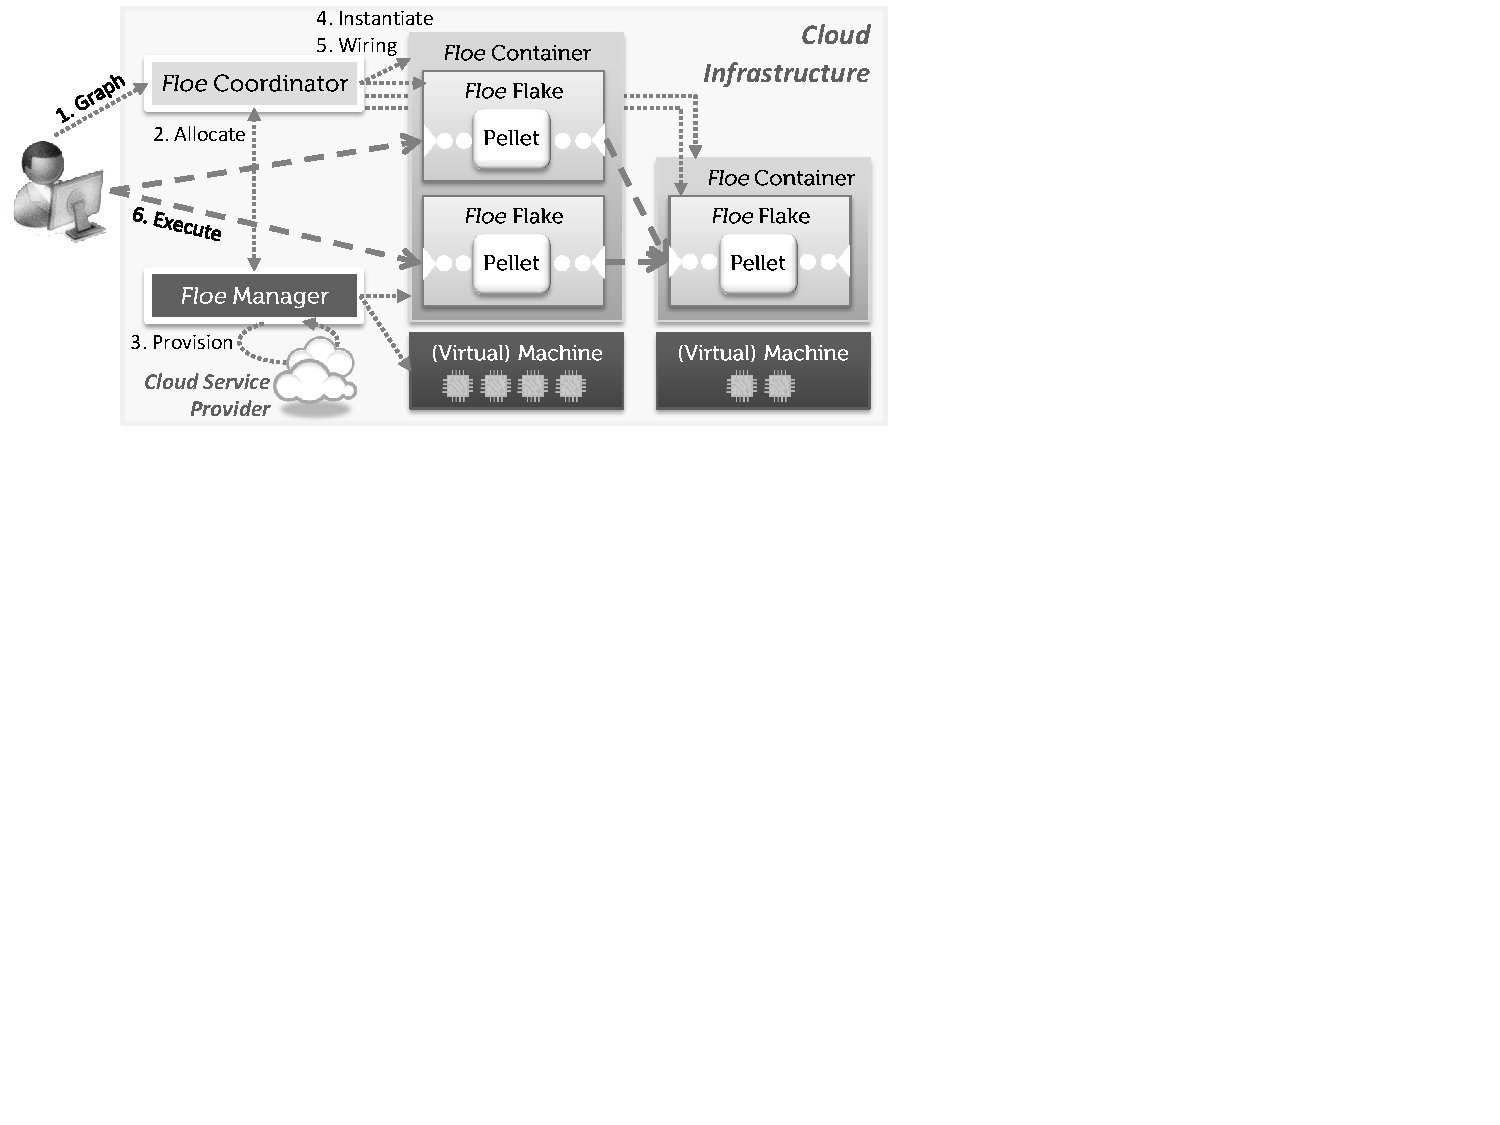
\includegraphics[width=0.5\columnwidth]{floe_arch}
\caption{\floe Architecture}
\label{fig:floe_arch}
\end{figure}

The \floe framework supports a graph based composition model to construct continuous dataflow applications. A programmer can define a reusable task, called Pellet, as a custom function with a set of typed input and output ports similar to the Action-Port model. The developer can then assemble several of these tasks to form a custom graph with output ports of upstream nodes connected to the compatible input ports of downstream nodes through a communication channel. Each task performs an operation on the incoming data, transforms it to the desired format and forwards the data to the downstream task. In addition, using the named input/output ports feature, the task can direct the data to a specific node in the downstream and thus achieve functionality similar to the MapReduce model.

The framework takes this application graph as input along with desired resource requirements and deploys it over a distributed environment. In addition, the framework continuously monitors the application execution to determine bottlenecks and allocate additional resources at runtime and hence provides scalable operations. It does so by monitoring the incoming data rate, the input queue, the task execution latency for each of the tasks in the application. If a bottleneck is observed, the framework increases the number of parallel instances of the given task and re-distributes the incoming data with appropriate load balancing strategies.


\section{Stream Clustering using Distributed LSH}
\label{sec:design}

We design our algorithm as an extension to the traditional online clustering algorithm (algo. \ref{algo:online}). In brief, the online algorithm processes each message at a time and assigns a cluster ID to that message. To do so, it first gets the list of all current clusters identfied so far (line 3) followed by distance calculation from the centroid of each of these clusters (lines 4-6). It then finds the cluster with minimum distance and if the distance is under a particular threshold, assigns the cluster to the message. Otherwise, it creates a new cluster for this data point (line 14). Further, it updates the cluster and modifies the centroid of the cluster based on this new data point. 

\begin{algorithm}
\SetAlgoLined
\KwData {Data Stream S, Candidate Selection function $\rho$, LSH parameter $N$}
\KwResult {For each item S[i] $\rightarrow$ out cluster ID}

	$C = \phi$ \;
	\For{each item S[i] in S}
	{
		%$\hat{C} = \rho(S[i],C)$\;
		$\hat{C} = \rho(S[i],C) = C$ \;
		
		
		\For{each cluster c in $\hat{C}$}
		{
			$D_i[c] = \delta{S[i],Centroid(c)}$\;
		}
		$D_{min} = min\lbrace D_i[c] | c \in \hat{C} \rbrace$\;
		$best_hash = \lbrace hash \in \hat{C,hash} | \delta(S[i],Centriod(\hat{c})) = D_{min} \rbrace$ \;
		$\hat{c} = \lbrace \hat{c} \in \hat{C} | \delta(S[i],Centriod(\hat{c})) = D_{min} \rbrace$ \;
		\eIf{$D_{min} \leq Threshold$}
		{
			$\hat{c} = \hat{c} \cup \lbrace S[i], best_hash \rbrace$ \;
		}
		{
			$newC = \lbrace S[i],  best_hsh \rbrace$ \;
			$ C = C \cup newC$ \;
		}
	}

\label{algo:online}
\caption{Online Clustering Algorithm}
\end{algorithm}

This algorithm finds the best clustering for the given threshold value, however there are a number of issues with respect to performance that needs to be addressed, specially in our scenario which involves continuous data streams. In particular, the need to consider all the existing clusters for comparison becomes a bottleneck. In addition, this algorithm processes a single message at a time, however, processing these messages can be done in parallel (as long as these messages are in different clusters). Also, we observe that the volume of stream data and hence the number of clusters is unbounded and hence the resources within a single machine may be insufficient and that the performance degrades over time as the system requirements for storage and processing keeps on increasing. To address all these issues we propose a distributed version of the online clustering algorithm using Locality sensitive hashing to improve the overall performance (algo \ref{algo:dlsh1}-\ref{algo:dlsh3}).

The idea behind the alogirthm is two fold, first, we use LSH to bound the number of clusters to be searched and, second, to distribute the clusters across various distributed nodes, each of these nodes can perform search locally in parallel. The buckets are distributed among the nodes using a standard hash function over the bucket id. for example using a standard mod function $Node id = Mod(bucket_{id}, \#nodes)$. This ensures equal distribution of the buckets among the distributed nodes. Note that, we do not need locality sensitive hashing to get the node id from the bucket id. The proposed algorithm is composed of three components (each of which is implemented as a Pellet task in FLOE) which can process the continuous stream of data. The first component, Bucketizer, uses LSH to find the potential clusters to be searched, it finds the corresponding nodes containing those clusters and dispatches it those nodes for searching. The cluster searcher, as the name indicates, gets a list of hashes from the bucketizer and searches the corresponding clusters to find the local best matching cluster. All these nodes perform this search in parallel and sends the result to the aggregator node, which in turn finds the global best. In addition, it has a feedback loop back to the cluster nodes which updates the corresponding cluster.

\begin{algorithm}
\SetAlgoLined 
\KwData {Data Stream S, Candidate Selection function $\rho$, LSH parameter $N$}
\KwResult {Dispatch each item S[i] to node containing the cluster}
	\For{each item S[i] in S}
	{
		%$\hat{C} = \rho(S[i],C)$\;
		$hashes = LSH(S[i],N)$ \;

		Parallel \For{each hash in $hashes$}
		{
			Node = FindNode(hash)\;
			Dispatch\_to\_clusterSearch(Node, hash, S[i])	
		}
	}				
\label{algo:dlsh1}
\caption{Bucketizer Component}
\end{algorithm}

\begin{algorithm}
Cluster Searcher\\
\SetAlgoLined 
\KwData {S[i], list of \textbf{\textit{hashes}} that belong to this node}
\KwResult {Find the best matching local cluster\\}

	$\hat{C} = search(hashes,C_{local})$\;
	\For{each cluster c in $\hat{C}$}
	{
		$D_i[c] = \delta{S[i],Centroid(c)}$\;
	}
	$D_{min_{local}} = min\lbrace D_i[c] | c \in \hat{C} \rbrace$\;
	$best\_hash = \lbrace hash \in \hat{C,hash} | \delta(S[i],Centriod(\hat{c})) = D_{min} \rbrace$ \;
	
	Dispatch\_to\_Aggregator($D_{min_{local}}, best\_hash, S[i], c.Id$)\;	
	
\label{algo:dlsh2}
\caption{Local Cluster Searcher}
\end{algorithm}


\begin{algorithm}
\SetAlgoLined 
\KwData {S[i], List<$D_{min_{local}}, best\_hash$, clusterId>}
\KwResult {Find Best Cluster}

	$D_{min} = min\lbrace D_{min_{local}} \rbrace$\;
	
	//corresponding to $D_{min}$\;
	$global\_best\_hash$\;
	$best_Cluster$\;

	$Node = findNode(global\_best\_hash)$\;
	\eIf{$D_{min} \leq Threshold$}
	{
		$dispatch(Node, global\_best\_hash, clusterId)$\;
	}
	{
		$newC = newCluster(nextClusterId)$\;
		$dispatch(Node, global\_best\_hash, clusterId)$\;
	}
	
\label{algo:dlsh3}
\caption{Aggregator}
\end{algorithm}



Figure \ref{fig:design} shows the design for a stream classification application built using the floe framework, specialized for text streams, that we have designed using this modified distributed LSH Scheme and is described below. Each node is a Floe task connected using communication channels for transferring messages. 

\begin{enumerate}
\item Task TC ( TweetCleaner ): This task is the first one to run. It processes tweet one by one and performs tasks such as tokenization, stop word removal, stemming.
\item Task BKT ( Bucketizer ): This node extracts the features from the tweet and performs locality sensitive hashing on those features to allocate the tweet to potential clusters with high probability of match with similar tweets. It then maps these clusters ids to node ids using a predefined hash function. It also passes the list of potential clusters ids ( buckets ) to search locally at each of these nodes.
\item Task CS ( ClusterSearcher ): It receives the tweet and list of potential clusters for that tweet which has a high probability of matching. It then searches only through those clusters to find the one with the minimum Euclidean distance. This distance is calculated from the Centroid of each of the potential clusters. This process is performed at each of the nodes with their respective tweets and their list of potential clusters. Each node only has local view of the clusters and hence there is a need to aggregate the results from various nodes to get the best match across all nodes.
\item Task AG ( Aggregator ): Each of the ClusterSearcher nodes sends the local best match cluster id along with the corresponding minimum distance to the aggregator node. The aggregator node then does the second level of comparison across all these received distances to find the global minimum distance and the corresponding cluster. Based on this information the aggregator sends feedback to corresponding CS node which then updates the Centroid of that particular cluster.
\end{enumerate}

\begin{figure}[!ht]
\centering
\includegraphics[width=0.6\columnwidth]{applications.pdf}
\caption{Stream Clustering using Distributed LSH over FLOE framework}
\label{fig:design}
\end{figure}


\section{Evaluation}
\label{sec:results}

\subsection{Data Set}
We will mainly be using the data set from Archive.org collected by Calufa. The database consists of 90 million tweets from 6 million users. The sql contains bio data, tweets, link information such as followers and following lists, location, profile name, users. The tweets are time stamped so we can use a stream generator to provide us with a stream. If we do not have data stream from other social networks, we plan to divide this data into multiple parts and generate streams from those data sets.
We have cleaned one more data set that we plan to use for testing and evaluating our system. We have downloaded and cleaned 96 million memes from MemeTracker dataset collected by SNAP at Stanford [4]. The memes are small in size suited for our analysis of small text documents.
We have one more twitter data set collected during a different time but comparatively smaller data set. The data set has also been used in [1]. It consists of tweets and their geographical locations. We can use it as another stream for our purposes.

\subsection{Experimental Setup}
We established a pseudo distributed system on a large multi core machine with the following configuration: 12 core, 24 GB RAM. To simulate the distributed system parameters we used socket communication for message passing instead of in-memory queues between various task processes. However our implementation can trivially be deployed on a distributed system without any change. We use the same system for evaluating Naive Stream Clustering as well as Distributed LSH based Stream Clustering. The preliminary results for both are shown in the next section.

We compare our approach against the Naive Stream Clustering. Naive Stream Clustering approach trivially compares the incoming tweet against all the buckets' centroids to find the best matching bucket. It is a non distributed (centralised) algorithm implementation. We compare our approach against the naive approach in two regards, first with respect to performance (i.e. average processing latency per message) and, second, with respect the accuracy of the approximate algorithm using F-measure as a metric.
\begin{figure}[!ht]
\centering
\includegraphics[width=0.8\columnwidth]{result1.pdf}
\caption{Average Latency Comparison: Naive Stream Clustering vs Distributed LSH Stream Clustering (with different no. of hash functions)}
\label{fig:result1}
\end{figure}
Figure \ref{fig:result1}. shows the average processing latency ( in milliseconds ) per tweet against the number of buckets at a constant data rate (1 tweet per second). We performed several experiments with varying number of LSH hash functions (N=10 to N=1000). As expected the average latency for the Naive Stream Clustering Approach increases linearly with number of buckets and hence it is not scalable for large data sets. Whereas, the latency for our proposed approach is independent of total buckets at a given data rate (1 tweet per second) for the given N. In addition, we observe that even with increasing the number of hash functions, in turn the number of clusters to search, we do not see much difference in performance (see N=10 and N=200 in fig. \ref{fig:result1}). This can be attributed to the fact that even though we are increasing the number of clusters to be searched, it will be distributed across various nodes and is performed in parallel. 



\begin{figure}[!ht]
\centering
\includegraphics[width=0.8\columnwidth]{result2.pdf}
\caption{F1-Score of DLSH with different number of hash functions}
\label{fig:result2}
\end{figure}

To compare the accuracy of the algorithm, we ran the naive algorithm and the proposed algorithm on the same dataset and obtained the clustered data. For each pair messages (tweets) in the data set, we find true positives (i.e. both the algorithms clustered the pair together), true negatives (i.e. both the algorithms put the pair in different clusters) and similarly false positives and false negatives if the result of the proposed algorithm is different from the naive algorithm. Figure \ref{fig:result2} shows the f-measure compared against the naive approach with differnt number of hash functions used in the algorithm. As expected, the algorithm performs better as we increase the number of hash functions and we achieved f1-score of 65% with N=1000 for the tweet database of about 100,000 tweets.



\section{Conclusion and Future Work}
\label{sec:future}
In this paper we proposed an extension to the online streaming algorithm to a distributed environment using LSH to reduce the search space. We implemented the system using, FLOE, a programming framework for continuous applications. Our experimental analysis shows the performance gains obtained by such a distributed system and the corresponding tradeoff with respect to accuracy. In future, further improvements can be made to analyze this tradeoff and develop parameter LSH schemes that take user preference into consideration to return variable number of hash values based on the preference instead of returning a fixed number every time. This can be used at runtime to fine tune the performance and accuracy of the algorithm with varying load on the system. Another interesting aspect to look into would be to determine the characteristics of algorithm and the efforts required to port these applications to the continuous (online) domain and to implement them as using the FLOE framework such that they can be published as open source Pellets and can reused across various applications.


\subsubsection*{References}

\small{

[1] 	Cheng Z., Caverlee J., Lee K., You Are Where You Tweet: A Content-Based Approach to Geo-locating Twitter Users. In Proceeding of the 19th ACM Conference on Information and Knowledge Management (CIKM), Toronto, Oct 2010. \newline
[2] Simmhan Y., Natarajan S., Kumbhare A., Prasanna V., Floe: Designing a Continuous Data Flow Engine for Dynamic Applications on the Cloud, tech report, University of Southern California (submitted). \newline
[3] Wadhwa, S.; Gupta, P.; , "Distributed Locality Sensitivity Hashing," Consumer Communications and Networking Conference (CCNC), 2010 7th IEEE , vol., no., pp.1-4, 9-12 Jan. 2010. \newline
[4] Jure Leskovec, Lars Backstrom, Jon Kleinberg, Meme-tracking and the Dynamics of the News Cycle. ACM SIGKDD International Conference on Knowledge Discovery and Data Mining (ACM KDD), 2009. \newline
[5] Daniel Barbara, Requirements for clustering data streams. ACM SIGKDD Explorations Newsletter Homepage archive
Volume 3 Issue 2, January 2002, Pages 23-27. \newline
[6] Madjid Khalilian, Norwati Mustapha, Data Stream Clustering: Challenges and Issues. Proceeding of the International MultiConference of Engineers and Computer Scienctists 2010 Vol I, IMECS 2010, March 17-19, 2010, Hong Kong. \newline
[7] Aggarwal, Charu C., et al. "A framework for projected clustering of high dimensional data streams." Proceedings of the Thirtieth international conference on Very large data bases-Volume 30. VLDB Endowment, 2004. \newline
[8] Steinbach, Michael, George Karypis, and Vipin Kumar. "A comparison of document clustering techniques." KDD workshop on text mining. Vol. 400. 2000. \newline
[9] Zhong, Shi. "Efficient online spherical k-means clustering." Neural Networks, 2005. IJCNN'05. Proceedings. 2005 IEEE International Joint Conference on. Vol. 5. IEEE, 2005.
[10] Kargupta, Hillol, et al. "Distributed clustering using collective principal component analysis." Knowledge and Information Systems 3.4 (2001): 422-448.
}

\end{document}
